\chapter{Case}


\section{Situation Report}

The overall objective off all parties involved in this case was to configure and develop a system that could receive \gls{sms}-reports. 

\begin{figure}
\centering
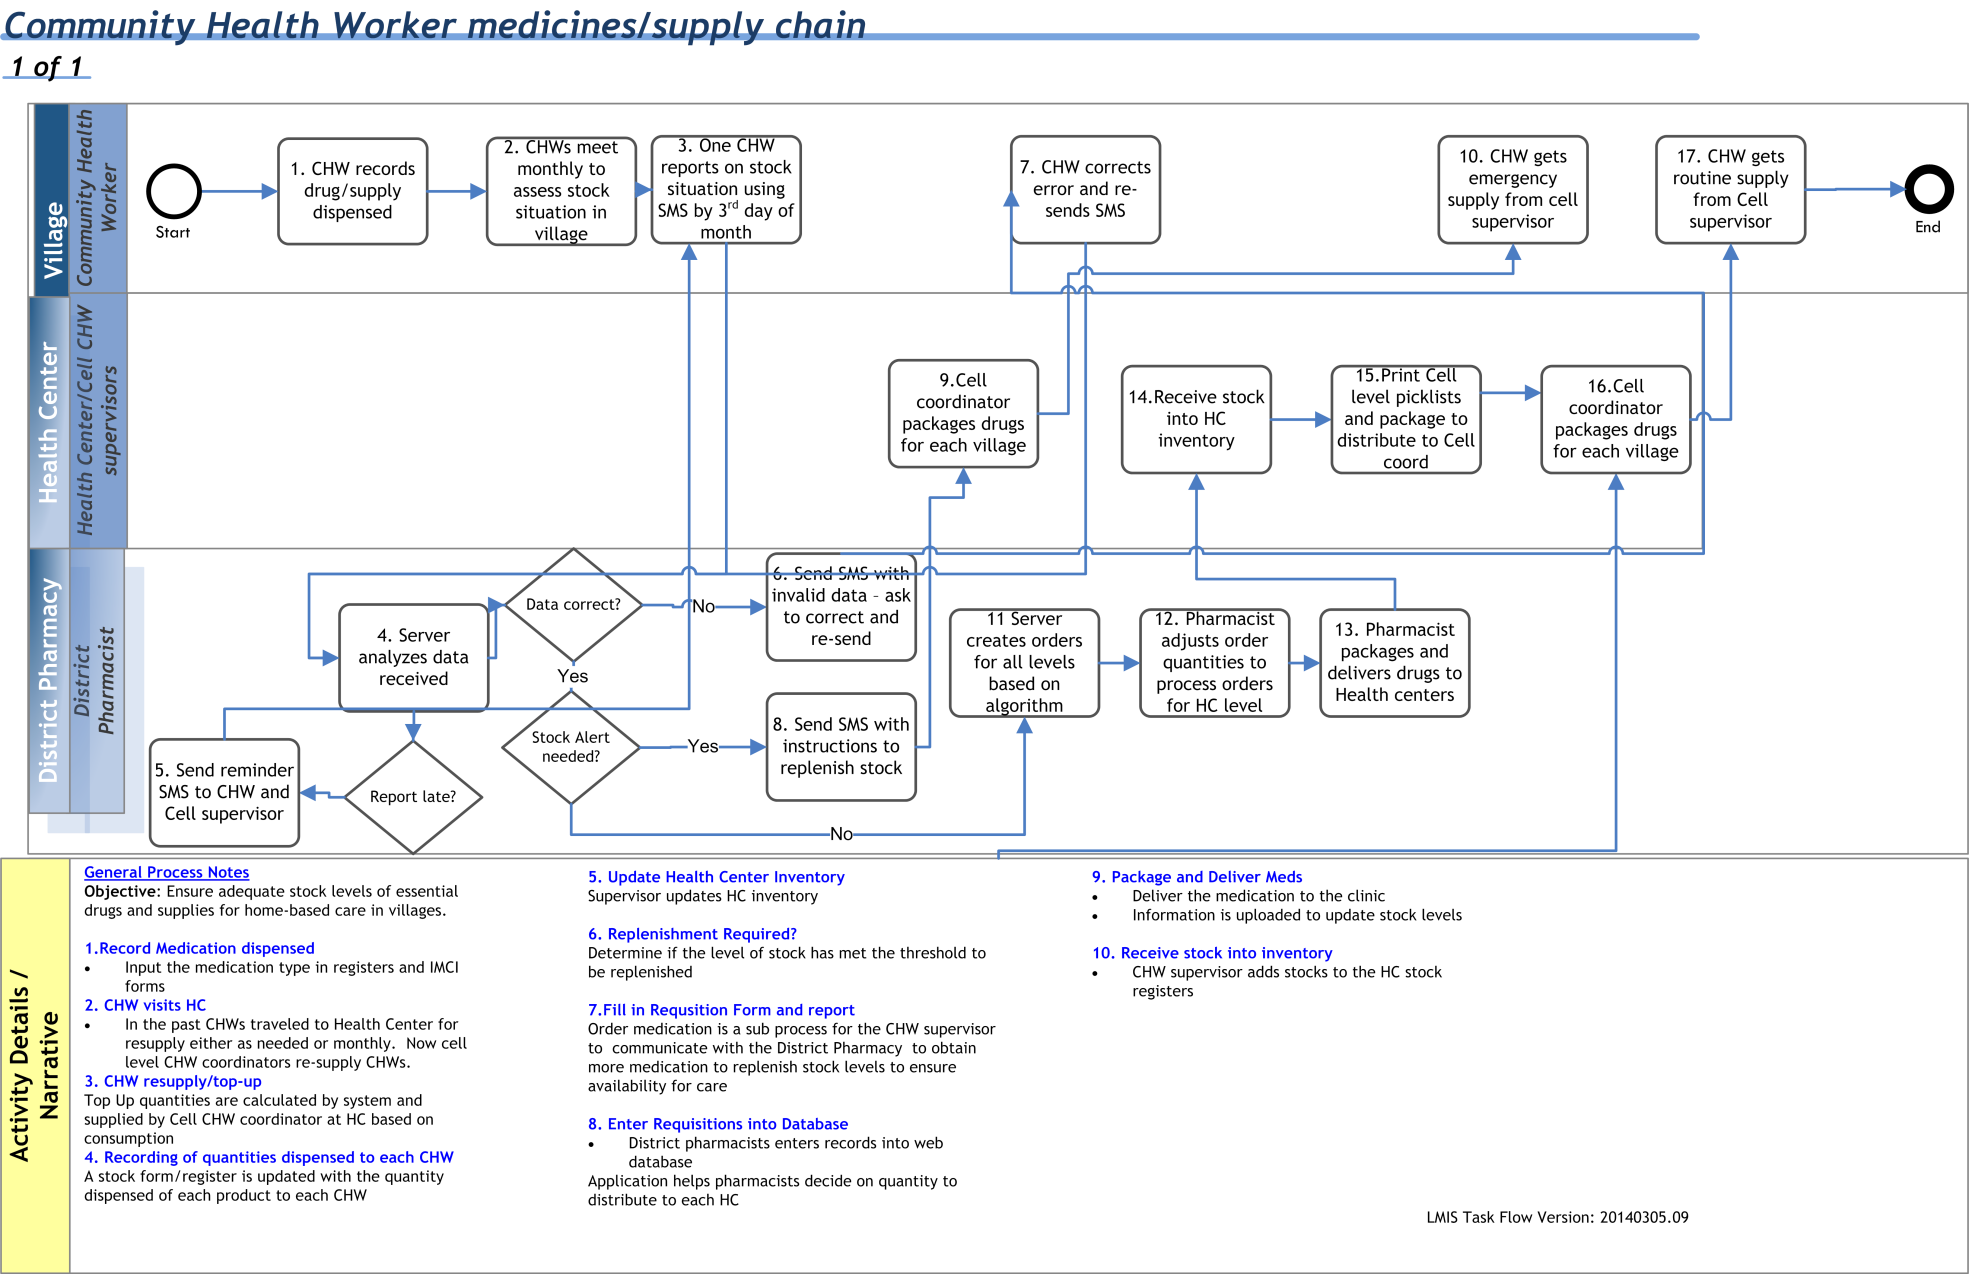
\includegraphics[width=\textwidth]{case/img/chwSupplyChainFuture}
\caption{\gls{chw} Supply Chain in the Future}
\label{chwSupplyChainPresent}
\end{figure}

\section{Diagnosis}

\subsection{Objectives}
We started out with four simple objectives. 

\begin{description}
\item[\#1:] Send SMS and email notifications based on rules.
\item[\#2:] Send SMS and email reminder if a report is more than 4 days delayed.
\item[\#3:] If user data does not map correctly user feedback should be provided.
\item[\#4:] A functional SMS based reporting system.
\end{description}

This was the basis for our case.

\subsection{Use Cases}

\begin{table}
	\centering
	\begin{tabular}{|p{5cm}|p{7cm}|}
		\hline
		\multicolumn{2}{|c|}{\textbf{Send SMS and Email Notifications}}\\
		\hline
		\textbf{Goal:} & Create orders\\
		\hline
		\textbf{Primary Actor:} & System\\
		\hline
		\multirow{3}{*}{\textbf{Secondary Actor:}}	& Cell CHW Supervisor \\
																								& HC CHW Supervisor \\ 
																								& District Pharmacist \\
		\hline
		\multirow{4}{*}{\textbf{Main Success Scenario:}}	& 1. CHW reports distributed and stock values. \\
																											& 2. System processes report. \\
																											& 3. System calculates essential drugs needed for each level. \\
																											& 4. System sends orders to cell, sector and district. \\
		\hline
		\textbf{Extensions:} & \\
		\hline
	\end{tabular}
	\caption{Textual Use Case: Send SMS and Email Notifications}
	\label{tab:notifications}
\end{table}


\begin{table}
	\centering
	\begin{tabular}{|p{5cm}|p{7cm}|}
		\hline
		\multicolumn{2}{|c|}{\textbf{Send SMS and Email Reminders}}\\
		\hline
		\textbf{Goal:} & Send reminder \\
		\hline
		\textbf{Primary Actor:} & System \\
		\hline
		\multirow{2}{*}{\textbf{Secondary Actor:}}	& CHW \\
																								& Cell CHW Supervisor \\
		\hline
		\multirow{5}{*}{\textbf{Main Success Scenario:}}	& 1. CHW misses report deadline. \\
																											& 2. 5 days goes by. \\
																											& 3. System sends reminder by email and SMS. \\
																											& 4. Another 5 days goes by. \\
																											& 5. System sends reminder by email and SMS. \\
																											
		\hline
		\textbf{Extensions:} & \\
		\hline
	\end{tabular}
	\caption{Textual Use Case: Send SMS and Email Reminders}
	\label{tab:reminders}
\end{table}


\begin{table}
	\centering
	\begin{tabular}{|p{5cm}|p{7cm}|}
		\hline
		\multicolumn{2}{|c|}{\textbf{Send Report Feedback}} \\
		\hline
		\textbf{Goal:} & Process SMS message\\
		\hline
		\textbf{Primary Actor:} & System \\
		\hline
		\textbf{Secondary Actor:} & Community Health Worker \\
		\hline
		\multirow{6}{*}{\textbf{Main Success Scenario:}}	& 1. CHW reports data incorrectly by SMS. \\
																											& 2. System receives SMS. \\
																											& 3. SMS triggers feedback message. \\
																											& 4. CHW corrects message and re-sends report. \\
																											& 5. System processes SMS. \\
																											& 6. System updates database. \\
		\hline
		\textbf{Extensions:} & \\
		\hline
	\end{tabular}
	\caption{Textual Use Case: Send Report Feedback}
	\label{tab:feedback}
\end{table}

\begin{table}
	\centering
	\begin{tabular}{|p{5cm}|p{7cm}|}
		\hline
		\multicolumn{2}{|c|}{\textbf{Report Using SMS}}\\
		\hline
		\textbf{Goal:} & Update Database \\
		\hline
		\textbf{Primary Actor:} & Community Health Worker\\
		\hline
		\textbf{Secondary Actor:} & System \\
		\hline
		\multirow{5}{*}{\textbf{Main Success Scenario:}}	& 1. CHW reports stock and distributed values of essential drugs. \\
																											& 2. System receives SMS. \\
																											& 3. System processes SMS. \\
																											& 4. System updates database. \\
																											& 5. System sends confirmation SMS to CHW. \\
		\hline
		\textbf{Extensions:} & \\
		\hline
	\end{tabular}
	\caption{Textual Use Case: Report Using SMS}
	\label{tab:smsreport}
\end{table}

Based on the four objectives we made four use cases that was supposed to represent each one. Objective \#1 would be represented with use case \ref{tab:notifications}, objective \#2 with \ref{tab:reminders}, \#3 with \ref{tab:feedback} and \#4 with \ref{tab:smsreport}. These use cases worked as guidelines for our further work. They were not updated later on, because of the continuous updated requirements from \gls{chd} and other co-workers. That is one of the key characterizations of this project. The requirements kept on updating as more and more people got involved in the process. The more progress we made the less progress we made. As the project was coming more and more realized, more interest were made to the project, and more requirements were added. There were a kind of common understanding in the team. Once you got the picture, you didn't need to operate on a model anymore. Everyone kinda knew what needed to be done. The result of the diagnosis were essentially a clarification of what we were supposed to do and who are involved. The clients are \gls{chd}. A meeting took place and a list of contact information was exchanged. The users of the system are \gls{chw}'s, Cell \gls{chw} Supervisors, \gls{hc} \gls{chw} Supervisors and District Pharmacists. The basic idea is that the \gls{chd} would like to have \gls{hmis} make a system that enables \gls{chw}'s to report using \gls{sms} and based on this have automatic generated orders sent to the \gls{hc}'s and District Pharmacists.

\section{Planning}

Our planning phase became somewhat glued together with the intervention. And continually altered. New problems were made visible by the interventions we made, and took us back to the planning phase. Making it very difficult to follow the action research model. In a perfect world, it is possible to plan everything to the point, but in our case new knowledge about the system was discovered along with our interventions and in turn, our plans had to be changed. 

\begin{figure}
\centering
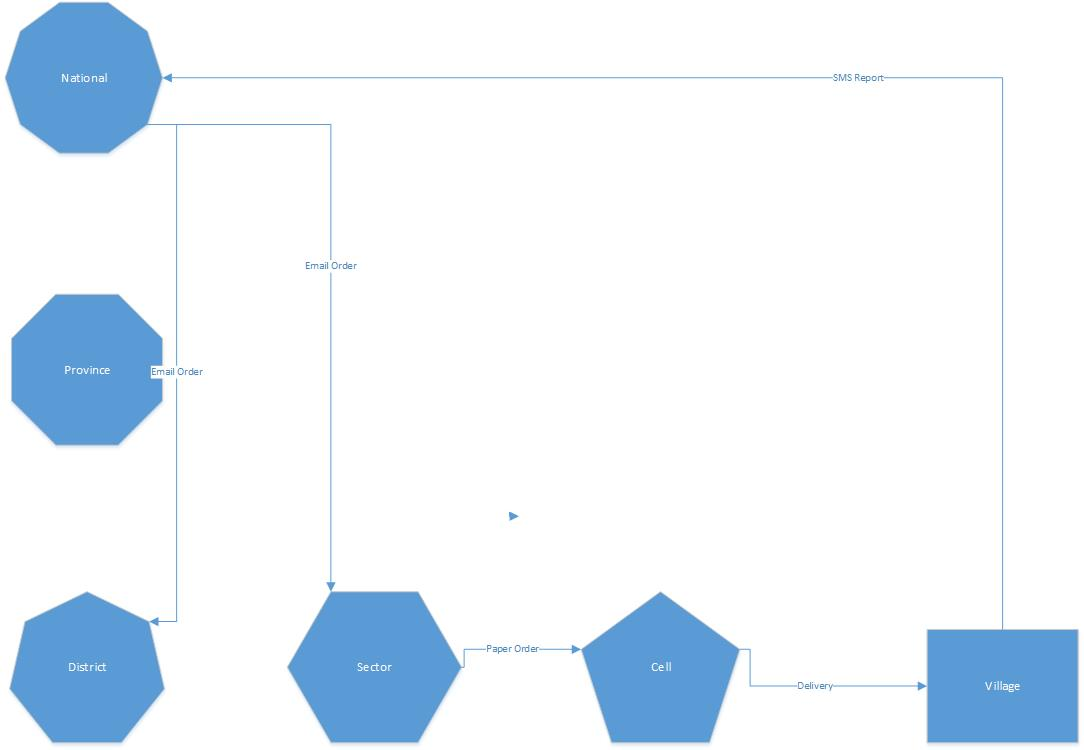
\includegraphics[width=\textwidth]{case/img/orderFlow}
\caption{Flow of Orders}
\label{fig:chworder}
\end{figure}

\section{Intervention}

\subsection{Setting up the Test Environment}
Our initial idea was to set up a \gls{dhis2} instance for testing purposes. This made it possible for us to check if our objectives was in some way already met with the functionality of \gls{dhis2}. We knew that \gls{dhis2} already supported \gls{sms} reporting, but it had never been tested. This was essentially what we did. Configured \gls{dhis2} to support our case. Turned out that objective \#3 and \#4 was already met with just configuring \gls{dhis2}. One thing that we did not think about that became a problem later was the translation of the feedback messages. \gls{chw}'s do not generally speak English, but the local language kinyarwanda. Fortunately, the translation of the messages was possible in the next version of \gls{dhis2}, so the objective was still met. 

\subsection{Setting up the mobile instance}
We sat up the \gls{dhis2} instance at the \gls{ndc}. This is server that the \gls{chw}'s will send their reports to. This process was very straight forward. The problem with having our instance running at a different location is that we have less control of our system. Now we have to go through another team to make certain changes to the system. Actually just slows down the whole process. Setting up the mobile instance made our plans more real and allowed us to show our work in real life. 


\subsection{User Importer}
The user importer was made in order to import user from a csv file. \gls{dhis2} did not support automatically generating usernames and passwords for bulk users. Therefore we needed a program to do this for us. The down side of this approach is that all the users of the system are not included in the process of creating user accounts. This by passes the \gls{hisp} philosophy of including local users in the system. Users may therefore have user accounts they are not aware of. Making the the users feel less ownership of the system. Despite of this we decided to take this approach.The amount of resources spent on manually register all the users would be to vast. 	

\begin{figure}
\centering
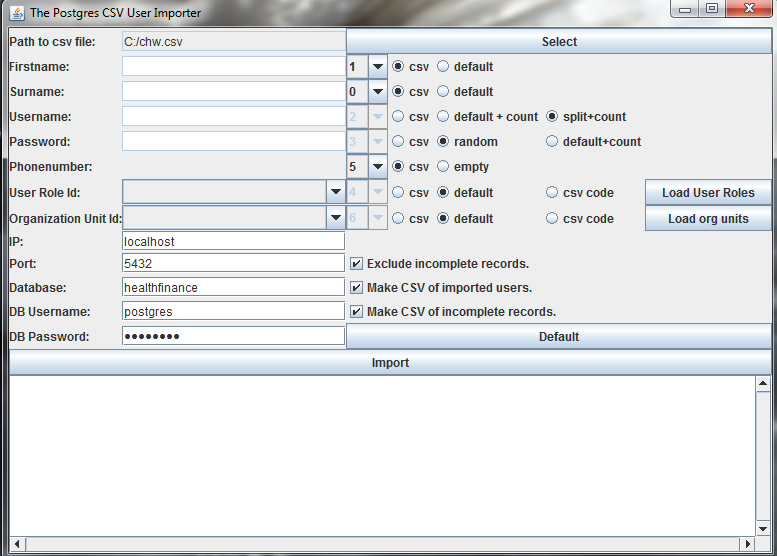
\includegraphics[width=\textwidth]{case/img/userImporterScreenShot}
\caption{Screen Shot of the User Importer}
\label{fig:screenUser}
\end{figure}

The user importer creates user accounts based on firstname, surname, village and phonenumber. After the user accounts are created they are able to send in \gls{sms}-reports based on the village they work from. 

\subsection{Re-Supply Algorithm}

\begin{equation}
stk_{n} = stk_{n-1} + rcd_{n} - disp_{n}
\end{equation}

\begin{eqnarray}
reorder_{n} & = & (amc_{n} \cdot 2) - stk_{n} \\
amc_{n} & = & \frac{disp_{n-2} + disp_{n-1} + disp_{n}}{3} \\
disp_{n} & = & stk_{n-1} + rcd_{n} - stk_{n} \\
disp_{n-1} & = & stk_{n-2} + rcd_{n-1} - stk_{n-1} \\
disp_{n-2} & = & stk_{n-3} + rcd_{n-2} - stk_{n-2}
\end{eqnarray}


\begin{description}
\item[$\mathbf{reorder_{n}}$]
This variable represents the quantity of how much is needed at the next re-supply of one village. $n$ in this case represents the last month. If in May, it represents reorder quantity for the end of month of April.
\item[$\mathbf{amc_{n}}$]
Represents the average monthly consumption based on the last 3 months in one village. I in May, that would be the average monthly consumption based on February, March and April.
\item[$\mathbf{disp_{n}}$]
This variable is calculated based on the the values reported and is the number of items distributed by one village during one month.
\item[$\mathbf{stk_{n}}$]
The quantity in stock at the end of the month of one village. Usually reported within 1--5 days into the next month it represents. Stock in April is usually reported between 1st and 5th of May.
\item[$\mathbf{rcd_{n}}$]
This variable is the sum of items received in one village during the month it represents. If a \gls{chw} receives 10 condoms 2nd of April, it should be reported the same day. If a village receives another 10 condoms the 13th of April, that should also be reported the same day it is received. $rcd_{n}$ for April would then be the sum of those values, 20.
\begin{equation}
rcd_{n} = \sum_{k = 1}^{j} rcd_{n,k}
\label{eq:received}
\end{equation}.
A more mathematical description in equation \ref{eq:received}, where j represents the number of days in the month.
\end{description}

\subsection{The Essential Predictore}
In order to generate the threshold values to send reminders from we chose to make a small application to run the algorithm. The application updates the database directly. The funny thing is that this was the only way we knew how to get our result, despite the support we had. The developer team from Oslo has offer the competence we needed, but due to the time frame we decided that we needed to build this application with SQL and JAVA. The application was kind of split in two. One of the team members at \gls{hmis} had a strong familiarity with databases and I had some JAVA experience. The core of the application was made in SQL, then it was wrapped inside a JAVA-\gls{gui}.

\begin{figure}
\centering
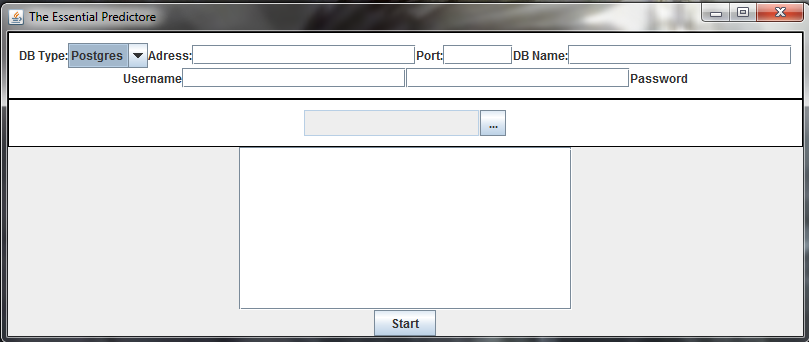
\includegraphics[width=\textwidth]{case/img/essentialPredictoreScreenShot}
\caption{Screen Shot of the Essential Predictore}
\label{fig:essPred}
\end{figure}

The collaboration in this application is something worth taking note of. Neither one of the team member knew exactly what the other was doing. The application was in fact copy-pasted together after making the the \gls{gui} and SQL-functionality separately. The application realizes the re-supply algorithm in a JAVA application and works with \gls{dhis2}. So all the tools from \gls{dhis2} could be taken advantage of. 